\documentclass[twoside]{book}
\newif\ifpdf
\ifx\pdfoutput\undefined
\pdffalse % we are not running PDFLaTeX
\else
\pdfoutput=1 % we are running PDFLaTeX
\pdftrue
\fi
%\usepackage{times}
%\usepackage{amsmath}
\usepackage{calc}
\usepackage[latin1]{inputenc}
\usepackage{FFF}
\usepackage{amsfonts}
\usepackage{amsmath}
\usepackage{hyperref}
\usepackage{FFF}
\usepackage{makeidx}
\usepackage{color}
\usepackage{multicol}
\usepackage{graphicx}
%\usepackage{dessin}
\topmargin -1.54cm
\oddsidemargin 0cm   %marge a 2 cm
\evensidemargin 0cm  %marge a 2 cm
\newcommand{\indente}{\hbox to \parindent {\hss}}
\parindent 0cm
\headsep 0.5cm
\topskip .5cm
\footskip 1cm
\headheight 1.0cm
\textwidth  16.5cm
%  \parindent 0cm
\textheight 24cm
\def\freefempp{\texttt{freefem++ }}
\def\textRed{\color{red}}
\def\textBlack{\color{black}}
\def\Blue#1{\textcolor{blue}{#1}}
\def\Black#1{\textcolor{black}{#1}}
\def\Red#1{\textcolor{red}{#1}}
\def\Magenta#1{\textcolor{magenta}{#1}}
\def\hin{\hbox{ in }}
\def\hon{\hbox{ on }}
\def\Cpp{\texttt{C++~}}
\def\R{\mathrm{I\!R}}
\def\example{\textbf{Example:}}
\def\eq#1{\Blue{\[#1\]}}
\def\R{\mathbb{R}}
\def\Z{\mathbb{Z}}
\def\itemtt[#1]{ \item[\texttt{#1}]}
\def\plot[#1]#2#3{\begin{figure}[hbt]
\begin{center}
    \includegraphics*[#1]{#2}
\end{center}
\caption{\label{#2} #3}
\end{figure}
}
\def\Ostream{\texttt{ostream}}
\def\Istream{\texttt{istream}}
\def\Bool{\texttt{bool}}
\def\Real{\texttt{real}}
\def\Int{\texttt{int}}
\def\vecttwo#1#2{\left|\begin{smallmatrix} #1 \\ #2 \end{smallmatrix}\right.}
\def\vdeux(#1,#2){\left|\begin{smallmatrix} #1 \\ #2 \end{smallmatrix}\right.}
\def\HLINE#1{\hbox to \hsize {#1}}
\def\twoplot[#1]#2#3#4#5{
\begin{figure}[hbt]
\begin{multicols}{2}
\begin{center}
    \includegraphics*[#1]{#2}
    \caption{\label{#2} #4}
\end{center}
\begin{center}
    \includegraphics*[#1]{#3}
    \caption{\label{#3} #5}
\end{center}
\end{multicols}
\end{figure}
}% end twoplot macro
\newtheorem{remark}{\textbf{Remark}}
\newtheorem{bug}{\textbf{Bug:}}
\newtheorem{proposition}{\textbf{Proposition}}
\newtheorem{algorithm}{\textbf{Algorithm}}
\newenvironment{ttlist}
   {\begin{list}{}{\renewcommand{\makelabel}[1]{\texttt{##1}\hfil}%
        \setlength{\labelwidth}{3cm}
        \setlength{\leftmargin}{\labelwidth+\labelsep}
    }}%
   {\end{list}}


\begin{document}
\graphicspath{{./}{plots/}}
\ifpdf
\DeclareGraphicsExtensions{.pdf, .jpg, .tif}
\else
\DeclareGraphicsExtensions{.eps,.ps, .jpg}
\fi

\let\subsubsection\subsection
\let\subsection\section
\let\section\chapter


%\subsubsection{Schwarz-overlap.edp}
\label{schwarz-overlap}
To solve 
\eq{ -\Delta u =f,\; \hin\Omega=\Omega_1\cup\Omega_2\quad u|_\Gamma=0}
the Schwarz algorithm  runs like this
\eq{
    -\Delta u^{m+1}_1=f\hin\Omega_1\quad
    u^{m+1}_1|_{\Gamma_1}=u^m_2
 }
\eq{
    -\Delta u^{m+1}_2=f\hin\Omega_2\quad
    u^{m+1}_2|_{\Gamma_2}=u^m_1
}
 where $\Gamma_i$ is the boundary of $\Omega_i$ and on the
condition that $\Omega_1\cap\Omega_2\ne\emptyset$ and that $u_i$
are zero at iteration 1.
\\\\
Here we take $\Omega_1$ to be a quadrangle, $\Omega_2$ a disk and
we apply the algorithm starting from zero.
\begin{figure}[hbt]
\HLINE{\hss
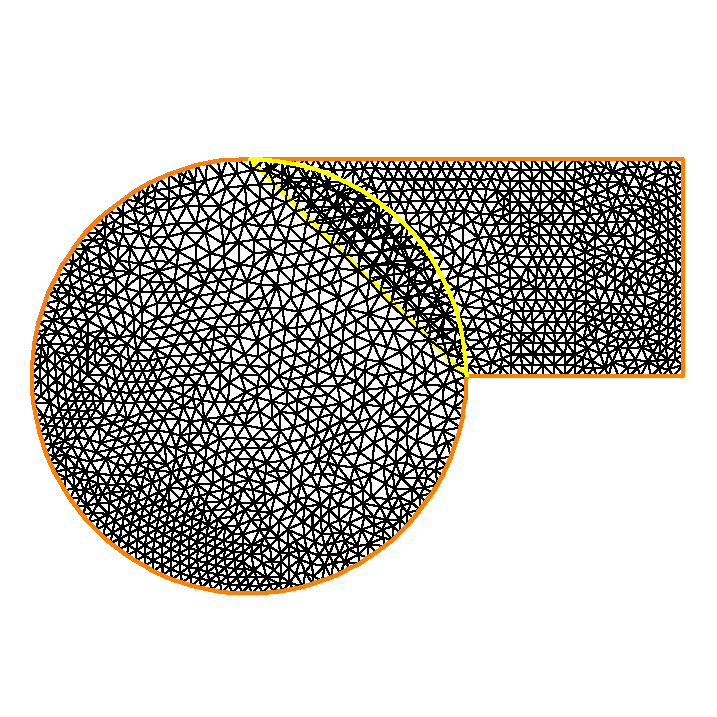
\includegraphics[width=6cm]{schwarz-th} \hss}
\caption{ The 2 overlapping mesh \texttt{TH} and \texttt{th}  }
\end{figure}

 \bFF

int inside = 2;  //  inside boundary
int outside = 1; //  outside boundary
border a(t=1,2){x=t;y=0;label=outside;};
border b(t=0,1){x=2;y=t;label=outside;};
border c(t=2,0){x=t ;y=1;label=outside;};
border d(t=1,0){x = 1-t; y = t;label=inside;};
border e(t=0, pi/2){ x= cos(t); y = sin(t);label=inside;};
border e1(t=pi/2, 2*pi){ x= cos(t); y = sin(t);label=outside;};
int n=4;
mesh th = buildmesh( a(5*n) + b(5*n) + c(10*n) + d(5*n));
mesh TH = buildmesh( e(5*n) + e1(25*n) );
plot(th,TH,wait=1);  //  to see the 2 meshes
\eFF

The space  and problem definition is :   
\bFF

fespace vh(th,P1);
fespace VH(TH,P1);
vh u=0,v; VH U,V;
int i=0;

problem PB(U,V,init=i,solver=Cholesky) = 
    int2d(TH)( dx(U)*dx(V)+dy(U)*dy(V) )
  + int2d(TH)( -V) + on(inside,U = u)  + on(outside,U= 0 ) ;
problem pb(u,v,init=i,solver=Cholesky) =
    int2d(th)( dx(u)*dx(v)+dy(u)*dy(v) )
  + int2d(th)( -v) + on(inside ,u = U) + on(outside,u = 0 ) ;
\eFF

 The  calculation loop: 
\bFF

for ( i=0 ;i< 10; i++)
{
   PB;
   pb;
   plot(U,u,wait=true);
};
\eFF



\begin{figure}[hbt]
\HLINE{\hss
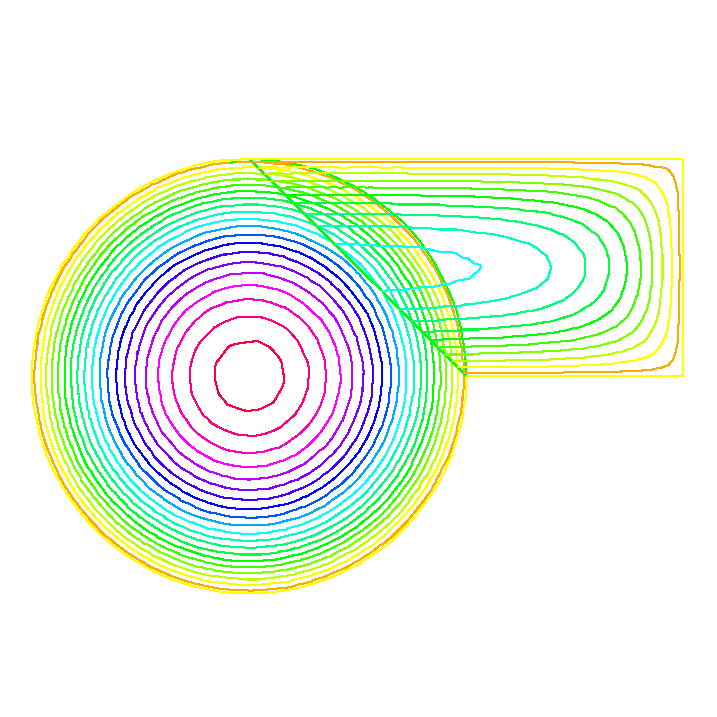
\includegraphics[width=6cm]{schwarz-u0} 
\hss
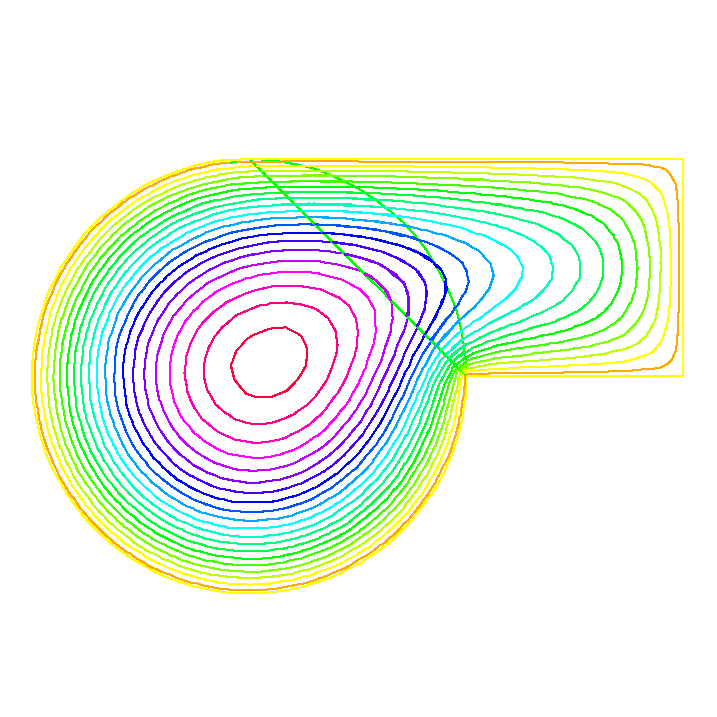
\includegraphics[width=6cm]{schwarz-u} }
\caption{  Isovalues of the solution at  iteration 0  and iteration 9}
\end{figure}



\end{document}